% Flow chart of the automatic initial guess (AUTO_GUESS.md).
% Compile: pdflatex flowchart.tex ; then rasterize to flowchart.png.
\documentclass[tikz,border=6pt]{standalone}
\usetikzlibrary{arrows.meta,positioning}
\begin{document}
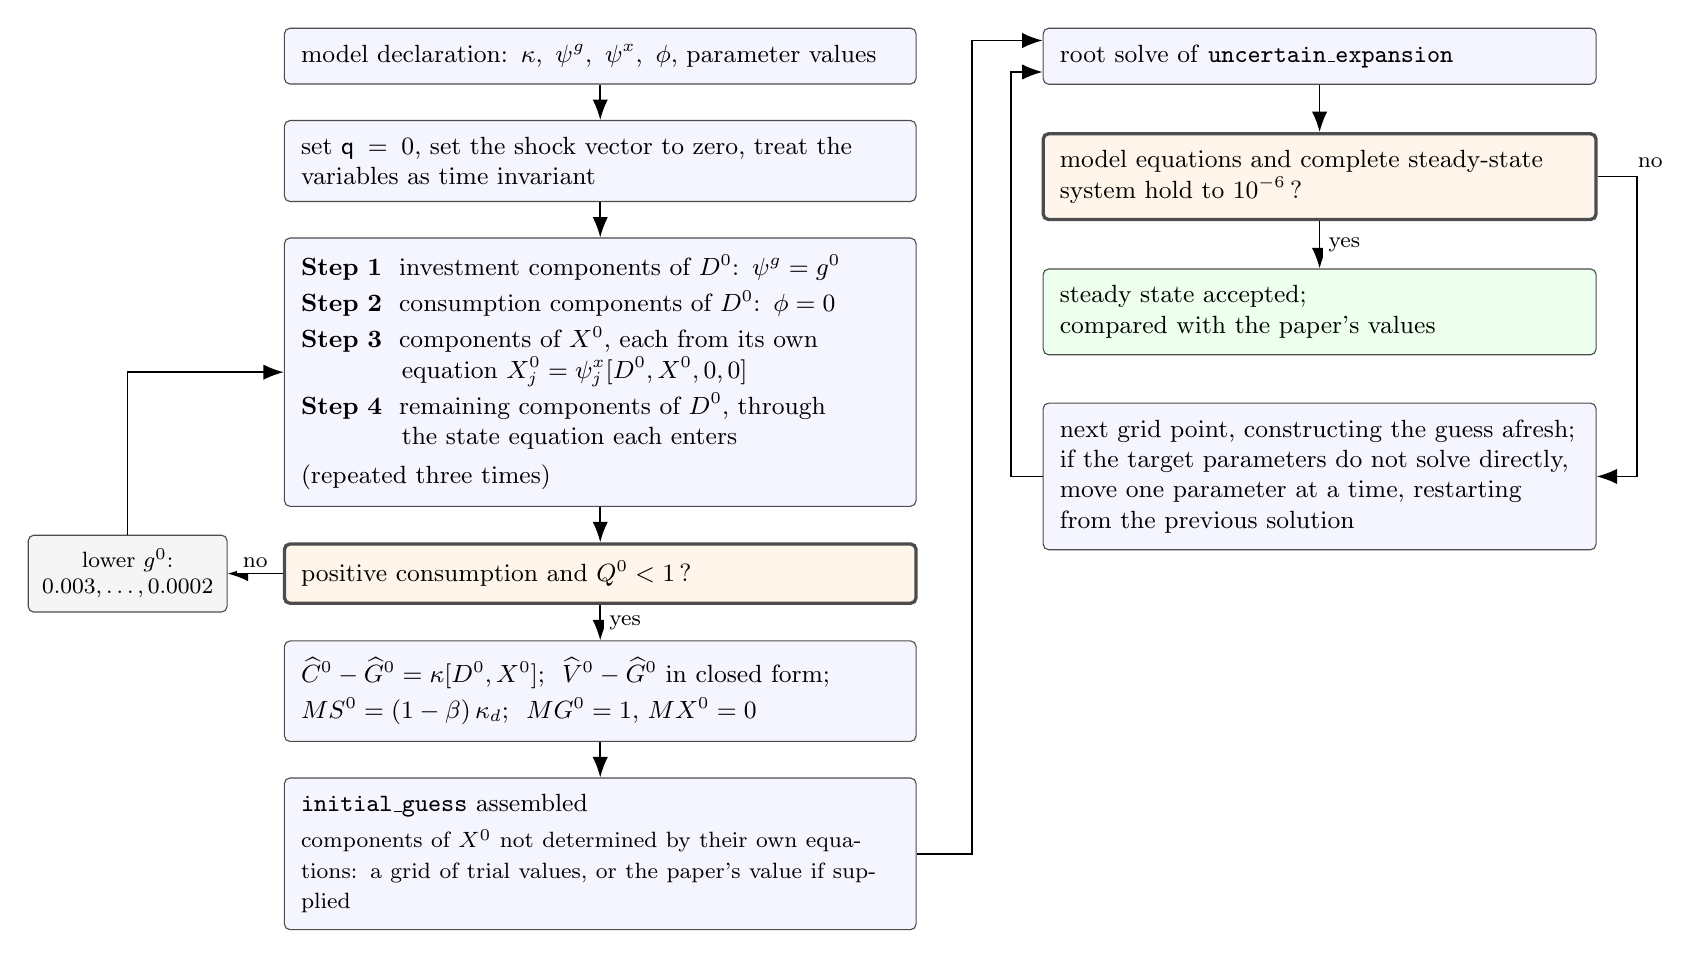
\begin{tikzpicture}[
  font=\small,
  box/.style={rectangle, rounded corners=2pt, draw=black!70, fill=blue!4,
              align=left, inner sep=6pt, text width=7.6cm},
  dec/.style={rectangle, rounded corners=2pt, draw=black!70, very thick,
              fill=orange!8, align=left, inner sep=6pt, text width=7.6cm},
  fin/.style={rectangle, rounded corners=2pt, draw=black!70, fill=green!7,
              align=left, inner sep=6pt, text width=6.6cm},
  rbox/.style={rectangle, rounded corners=2pt, draw=black!70, fill=blue!4,
              align=left, inner sep=6pt, text width=6.6cm},
  rdec/.style={rectangle, rounded corners=2pt, draw=black!70, very thick,
              fill=orange!8, align=left, inner sep=6pt, text width=6.6cm},
  lp/.style={rectangle, rounded corners=2pt, draw=black!70, fill=black!4,
             align=center, inner sep=5pt, font=\footnotesize},
  a/.style={-{Latex[length=2.6mm]}, semithick},
  lbl/.style={font=\footnotesize, inner sep=2pt, fill=white}
]

% ---------------- left column: construction ----------------
\node[box] (decl) {model declaration: $\kappa,\ \psi^g,\ \psi^x,\ \phi$, parameter values};
\node[box, below=4.5mm of decl] (det)
  {set $\mathsf q=0$, set the shock vector to zero, treat the variables as
   time invariant};
\node[box, below=4.5mm of det] (steps)
  {\textbf{Step 1}\ \ investment components of $D^0$: $\psi^g=g^0$\\[2pt]
   \textbf{Step 2}\ \ consumption components of $D^0$: $\phi=0$\\[2pt]
   \textbf{Step 3}\ \ components of $X^0$, each from its own\\
   \hspace*{1.28cm}equation $X_j^0=\psi_j^x[D^0,X^0,0,0]$\\[2pt]
   \textbf{Step 4}\ \ remaining components of $D^0$, through\\
   \hspace*{1.28cm}the state equation each enters\\[3pt]
   (repeated three times)};
\node[dec, below=4.5mm of steps] (feas)
  {positive consumption and $Q^0<1$\,?};
\node[lp, left=7mm of feas] (lower)
  {lower $g^0$:\\ $0.003,\dots,0.0002$};
\node[box, below=4.5mm of feas] (val)
  {$\widehat C^0-\widehat G^0=\kappa[D^0,X^0]$;\ \
   $\widehat V^0-\widehat G^0$ in closed form;\\[2pt]
   $MS^0=(1-\beta)\,\kappa_d$;\ \ $MG^0=1$,\ $MX^0=0$};
\node[box, below=4.5mm of val] (ig)
  {\texttt{initial\_guess} assembled\\[2pt]
   \footnotesize components of $X^0$ not determined by their own
   equations: a grid of trial values, or the paper's value if supplied};

% ---------------- right column: solve ----------------
\node[rbox, right=16mm of decl.north east, anchor=north west] (root)
  {root solve of \texttt{uncertain\_expansion}};
\node[rdec, below=6mm of root] (acc)
  {model equations and complete steady-state system hold to $10^{-6}$\,?};
\node[fin, below=6mm of acc] (done)
  {steady state accepted;\\ compared with the paper's values};
\node[rbox, below=6mm of done] (retry)
  {next grid point, constructing the guess afresh; if the target
   parameters do not solve directly, move one parameter at a time,
   restarting from the previous solution};

% ---------------- arrows ----------------
\draw[a] (decl) -- (det);
\draw[a] (det) -- (steps);
\draw[a] (steps) -- (feas);
\draw[a] (feas.west) -- node[lbl, above]{no} (lower.east);
\draw[a] (lower.north) |- (steps.west);
\draw[a] (feas) -- node[lbl, right=1pt]{yes} (val);
\draw[a] (val) -- (ig);
\draw[a] (ig.east) -- ++(7mm,0) |- ([yshift=2mm]root.west);
\draw[a] (root) -- (acc);
\draw[a] (acc) -- node[lbl, right=1pt]{yes} (done);
\draw[a] (acc.east) -- ++(5mm,0) node[lbl, above right=1pt and -2pt]{no} |- (retry.east);
\draw[a] (retry.west) -- ++(-4mm,0) |- ([yshift=-2mm]root.west);
\end{tikzpicture}
\end{document}
